\tikzstyle{input_neuron}=[circle,draw=red!50,fill=red!10,thick,minimum size=6mm]
\tikzstyle{hidden_neuron}=[circle,draw=blue!50,fill=cyan!10,thick,minimum size=1mm]
\tikzstyle{output_neuron}=[circle,draw=green!50,fill=green!20,thick,minimum size=1mm]
\tikzstyle{input}=[circle,draw=black!50,fill=black!20,thick,minimum size=1mm]

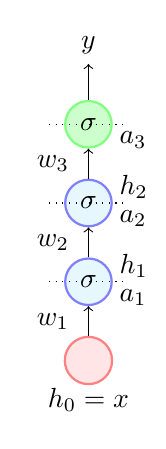
\begin{tikzpicture}

	\node [input_neuron] (neuron0) at (6,5)  {} ;
	\node (input0) at (6,4.5)  {$h_0=x$};
	\node (output0) at (6,9){$y$};
	
	\node [hidden_neuron] (neuron1) at (6,6)  {$\sigma$};
	\node [hidden_neuron] (neuron2) at (6,7)  {$\sigma$};
	\node [output_neuron] (neuron3) at (6,8)  {$\sigma$};
	
	%\draw [->] (input0) -- (neuron0);
	\draw [->] (neuron0) -- (neuron1);
	\draw [->] (neuron1) -- (neuron2);
	\draw [->] (neuron2) -- (neuron3);
	\draw [->] (neuron3) -- (output0); 
	%\draw [dotted] (5.5,5) -- (6.5,5);
	\draw [dotted] (5.5,6) -- (6.5,6);
	\draw [dotted] (5.5,7) -- (6.5,7);
	\draw [dotted] (5.5,8) -- (6.5,8);
	%\node[text width=0.01cm] at (6.4,4.8) {$a_1$};
	%\node[text width=0.01cm] at (6.4,5.2) {$h_1$};
	\node[text width=0.01cm] at (6.4,5.8) {$a_1$};
	\node[text width=0.01cm] at (6.4,6.2) {$h_1$};
	\node[text width=0.01cm] at (6.4,6.8) {$a_2$};
	\node[text width=0.01cm] at (6.4,7.2) {$h_2$};
	\node[text width=0.01cm] at (6.4,7.8) {$a_3$};
	%\node[text width=0.01cm] at (6.4,8.2) {$h_3$};
	
	\node (formula) at (5.55,5.5) {$w_1$};
	\node (formula) at (5.55,6.5) {$w_2$};
	\node (formula) at (5.55,7.5) {$w_3$};
	
\end{tikzpicture}